%iffalse
\let\negmedspace\undefined
\let\negthickspace\undefined
\documentclass[journal,onecolumn]{IEEEtran}
\usepackage{cite}
\usepackage{amsmath,amssymb,amsfonts,amsthm}
\usepackage{algorithmic}
\usepackage{graphicx}
\usepackage{textcomp}
\usepackage{xcolor}
\usepackage{txfonts}
\usepackage{listings}
\usepackage{enumitem}
\usepackage{mathtools}
\usepackage{gensymb}
\usepackage{comment}
\usepackage[breaklinks=true]{hyperref}
\usepackage{tkz-euclide} 
\usepackage{listings}
\usepackage{gvv}                                        
%\def\inputGnumericTable{}                                 
\usepackage[latin1]{inputenc}                                
\usepackage{color}                                            
\usepackage{array}                                            
\usepackage{longtable}                                       
\usepackage{calc}                                             
\usepackage{multirow}                                         
\usepackage{hhline}                                           
\usepackage{ifthen}                                           
\usepackage{lscape}
\usepackage{tabularx}
\usepackage{array}
\usepackage{float}
\usepackage{tikz}
\usetikzlibrary{arrows.meta}

\newtheorem{theorem}{Theorem}[section]
\newtheorem{problem}{Problem}
\newtheorem{proposition}{Proposition}[section]
\newtheorem{lemma}{Lemma}[section]
\newtheorem{corollary}[theorem]{Corollary}
\newtheorem{example}{Example}[section]
\newtheorem{definition}[problem]{Definition}
\newcommand{\BEQA}{\begin{eqnarray}}
\newcommand{\EEQA}{\end{eqnarray}}
\newcommand{\define}{\stackrel{\triangle}{=}}
\theoremstyle{remark}
\newtheorem{rem}{Remark}

% Marks the beginning of the document
\begin{document}
\bibliographystyle{IEEEtran}
\vspace{3cm}

\title{AE 2008 Q52-68}
\author{EE24BTECH11002 - Agamjot Singh}
\maketitle

\renewcommand{\thefigure}{\theenumi}
\renewcommand{\thetable}{\theenumi}

\begin{enumerate}
    \setcounter{enumi}{51}

    %Question52
    \item The geometrical features of a supercritical airfoil are

	\begin{enumerate}
		\item rounded leading edge, flat upper surface and high camber at the rear
		\item sharp leading edge, curved upper surface and high camber at the rear
		\item rounded leading edge, curved upper surface and no camber at the rear
		\item sharp leading edge, flat upper surface and no camber at the rear
	\end{enumerate}

    %Question53
    \item Which one of the following high lift device results in higher stalling angle?

	\begin{enumerate}
		\item split flap
		\item Fowler flap
		\item plain flap
		\item leading edge flap
	\end{enumerate}

    %Question54
    \item A turbofan engine has bypass ratio of 5 and a total mass flow rate of $120$ kg/s. The mass flow rate through the bypass duct is

	\begin{enumerate}
		\item $20$ kg/s
		\item $100$ kg/s
		\item $120$ kg/s
		\item $600$ kg/s
	\end{enumerate}


    %Question55
    \item A turbojet engine is operating with afterburner off. If the afterburner is switched on, then

	\begin{enumerate}
		\item both thrust and $sfc$ decrease
		\item thrust increases and $sfc$ decreases
		\item thrust decreases and $sfc$ increases
		\item both thrust and $sfc$ increase 
	\end{enumerate}

    %Question56
    \item A centrifugal compressor operates with a tip blade speed of $340$ m/s. The air leaves the impeller with a radial velocity of $88$ m/s. If the slip factor is $0.85$, the relative velocity of the blade tip is

	\begin{enumerate}
		\item $101.7$ m/s
		\item $120.3$ m/s
		\item $132.6$ m/s
		\item $135.8$ m/s
	\end{enumerate}

    %Question57
    \item An ideal ramjet engine is flying at a Mach number $M$. The exhaust gas static temperature at the outlet of the nozzle is $T_e$. The ambient static temperature is $T_{\alpha}$. Gas constant $R$ and specific heat ratio $\gamma$ do not vary through the ramjet. Assuming that nozzle exhaust static pressure is equal to the ambient pressure and fuel air ratio $f << 1$, the thrust per unit mass flow rate is

	\begin{enumerate}
		\item $\sqrt{\gamma R T_{\alpha}}\brak{\sqrt{\frac{T_e}{T_{\alpha}}}}$
		\item $\sqrt{\gamma R T_{\alpha}}\brak{\sqrt{\frac{T_e}{T_{\alpha}}} - 1}$
		\item $M\sqrt{\gamma R T_{\alpha}}\brak{\sqrt{\frac{T_e}{T_{\alpha}}} - 1}$
		\item $M\sqrt{\gamma R T_{\alpha}}\brak{\sqrt{\frac{T_e}{T_{\alpha}}}}$
	\end{enumerate}


    %Question58
    \item A $50$ percent degree of reaction axial flow turbine operates with a mean blade speed of $180$ m/s. The flow leaves the stator and enters the rotor at an angle of $60$ degrees to the axial direction. The axial velocity is $150$ m/s, and remains constant throughout the stage. THe turbine power per unit mass flow is

	\begin{enumerate}
		\item $29.76$ kJ/kg
		\item $41.12$ kJ/kg
		\item $58.33$ kJ/kg
		\item $61.13$ kJ/kg
	\end{enumerate}


    %Question59
    \item The chamber stagnation temperature inside a rocket motor is $T_e$. Only a convergent nozzle is used, and the flow at the exit of the nozzle is choked. Assume that the nozzle exhaust static pressure is equal to the ambient static pressure. Gas constant for exhaust gases is $R$ and ratio of specific heats is $\gamma$. The specific impulse of the rocket motor is

	\begin{enumerate}
		\item $\sqrt{\frac{2\gamma R T_e}{\gamma - 1}}$
		\item $\sqrt{\frac{\gamma R T_e}{\gamma - 1}}$
		\item $\sqrt{\frac{\gamma R T_e}{\gamma + 1}}$
		\item $\sqrt{\frac{2\gamma R T_e}{\gamma + 1}}$
	\end{enumerate}


    %Question60
    \item Air enters the combustor of a gas turbine engine at total temperature of $500$ K and leaves the combustor at total temperature of $1800$ K. If $c_p$ remains constant at $1.005$ kJ/kgK and heating value of the fuel used is $44$ MJ/kg, the fuel to air ratio is

	\begin{enumerate}
		\item $0.003$
		\item $0.012$
		\item $0.031$
		\item $0.074$
	\end{enumerate}


    %Question61
    \item The inital temperature sensitivity of burn rate of a solid rocket motor propellant is positive. If the inital temperature increases then 

	\begin{enumerate}
		\item thrust increases but burn time decreases
		\item thrust decreases and burn time decreases too
		\item thrust remains same but burn time increases
		\item thrust increases but burn time remains same
	\end{enumerate}


    %Question62
    \item An aircraft is cruising at a Mach number of $0.8$ at an altitude where the ambient static pressure is $95$ kPa. The diffuser exit total pressure is $140$ kPa. Assuming there is no change in the specific heat at constant pressure across the diffuser, and the ratio of specific heats is $1.4$, the adiabatic efficiency of the intake is

	\begin{enumerate}
		\item $0.988$
		\item $0.915$
		\item $0.722$
		\item $0.684$
	\end{enumerate}


    %Question63
    \item A parallelogram shaped plate of dimensions $'a'$ and $'b'$ as shown in the figure, is subjected to a uniform loading of normal stresses $\sigma_1$ and $\sigma_2$. The plate is in equilibrium for
	\begin{center}
	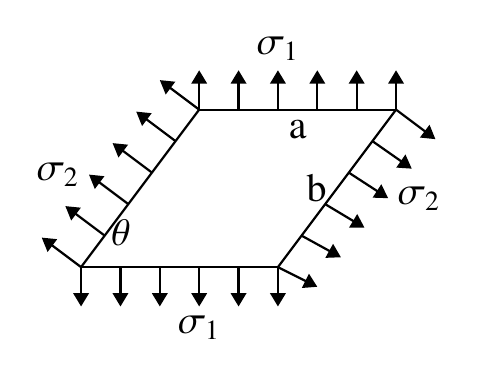
\begin{tikzpicture}[scale =0.5]
		\draw[black, thick] (0,0) -- (3,4);
		\node at (1, 0.3) [above] {\Large $\theta$};
		\draw[black, thick] (3,4) -- node[below] {\Large a} (8,4);
		\draw[black, thick] (8, 4) -- node[left] {\Large b} (5,0);
		\draw[black, thick] (5,0) -- (0,0);

		\draw [-Triangle, thick] (0, 0) -- (-1, 3/4);
		\draw [-Triangle, thick] (3/5, 4/5) -- (-1 + 3/5, 3/4 + 4/5);
		\draw [-Triangle, thick] (3/5 * 2, 4/5 * 2) -- (-1 + 3/5 * 2, 3/4 + 4/5 * 2);
		\node at (-1 + 3/5 * 2, 3/4 + 4/5 * 2) [left] {\Large $\sigma_2$};
		\draw [-Triangle, thick] (3/5 * 3, 4/5 * 3) -- (-1 + 3/5 * 3, 3/4 + 4/5 * 3);
		\draw [-Triangle, thick] (3/5 * 4, 4/5 * 4) -- (-1 + 3/5 * 4, 3/4 + 4/5 * 4);
		\draw [-Triangle, thick] (3/5 * 5, 4/5 * 5) -- (-1 + 3/5 * 5, 3/4 + 4/5 * 5);

		\draw [-Triangle, thick] (3, 4) -- (3, 5);
		\draw [-Triangle, thick] (4, 4) -- (4, 5);
		\draw [-Triangle, thick] (5, 4) -- (5, 5);
		\node at (5, 5) [above] {\Large $\sigma_1$};
		\draw [-Triangle, thick] (6, 4) -- (6, 5);
		\draw [-Triangle, thick] (7, 4) -- (7, 5);
		\draw [-Triangle, thick] (8, 4) -- (8, 5);

		\draw [-Triangle, thick] (8, 4) -- (8 + 1, 4 - 3/4);
		\draw [-Triangle, thick] (8 - 3/5, 4 - 4/5) -- (8 + 1 - 3/5, 4 - 3/4 * 2);
		\draw [-Triangle, thick] (8 - 3/5 * 2, 4 - 4/5 * 2) -- (8 + 1 - 3/5 * 2, 4 - 3/4 * 3);
		\node at (8 + 1 - 3/5 * 2, 4 - 3/4 * 3) [right] {\Large $\sigma_2$};
		\draw [-Triangle, thick] (8 - 3/5 * 3, 4 - 4/5 * 3) -- (8 + 1 - 3/5 * 3, 4 - 3/4 * 4);
		\draw [-Triangle, thick] (8 - 3/5 * 4, 4 - 4/5 * 4) -- (8 + 1 - 3/5 * 4, 4 - 3/4 * 5);
		\draw [-Triangle, thick] (8 - 3/5 * 5, 4 - 4/5 * 5) -- (8 + 1 - 3/5 * 5, 4 - 3/4 * 6);

		\draw [-Triangle, thick] (5, 0) -- (5, -1);
		\draw [-Triangle, thick] (4, 0) -- (4, -1);
		\draw [-Triangle, thick] (3, 0) -- (3, -1);
		\node at (3, -1) [below] {\Large $\sigma_1$};
		\draw [-Triangle, thick] (2, 0) -- (2, -1);
		\draw [-Triangle, thick] (1, 0) -- (1, -1);
		\draw [-Triangle, thick] (0, 0) -- (0, -1);
		
	\end{tikzpicture}
	\end{center}
	\begin{enumerate}
		\item any value of $\sigma_1$ and $\sigma_2$
		\item $\sigma_1 = \sigma_2 \cos{\theta}$
		\item $\sigma_2 = \sigma_1 \cos{\theta}$
		\item $\sigma_2 = \sigma_1$
	\end{enumerate}

    %Question64
    \item A column of solid circular cross-section and length $L$ can have various end conditions. Choose correct set that matches the end conditions $\brak{\text{listed in Group I}}$ with the corresponding effective length for buckling $\brak{\text{listed in Group II}}$.

	\begin{table}[h!]
		\centering
		\begin{tabular}[12pt]{ |c| c|}
    \hline
    \textbf{Variable} & \textbf{Description}\\ 
    \hline
	$\vec{A}$ & Point to be found\\
    \hline
	$\vec{B}$ & $(0, 0)$ point\\
    \hline
	$\vec{C}$ & $(6, 0)$ point\\
    \hline
	$\vec{\angle \vec{ABC}}$ & $60 \degree$\\ 
    \hline
    \end{tabular}
		\label{taba1.q64}
	\end{table}

	\begin{enumerate}
		\item $P - 3, Q - 1, R - 4, S - 2$
		\item $P - 4, Q - 1, R - 2, S - 3$
		\item $P - 2, Q - 1, R - 3, S - 4$
		\item $P - 3, Q - 1, R - 2, S - 4$
	\end{enumerate}

    %Question65
    \item A thin walled tube of circular cross-section with mean radius $r$ has a central web which divides it into two symmetric cells as shown. A torque $M$ is acting on the section. The shear flow $q$ in the central web is
	\begin{center}
	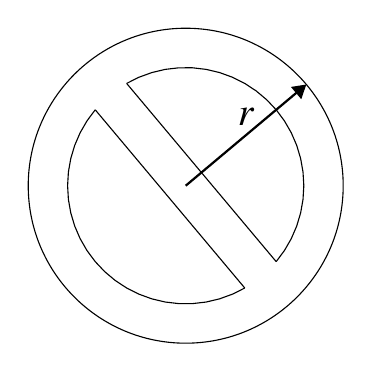
\begin{tikzpicture}
		\draw (0,0) circle (2cm);
		\draw [domain=-40:120] plot ({1.5*cos(\x)}, {1.5*sin(\x)});
		\draw [domain=140:300] plot ({1.5*cos(\x)}, {1.5*sin(\x)});

		\draw ({3/2*cos(-40)}, {3/2*sin(-40)}) -- ({3/2*cos(120)}, {3/2*sin(120)});
		\draw ({3/2*cos(140)}, {3/2*sin(140)}) -- ({3/2*cos(300)}, {3/2*sin(300)});

		\draw [-Triangle, thick] (0, 0) -- ({2*cos(40)}, {2*sin(40)});
		\node at ({cos(40)}, {sin(40)}) [above] {\Large $r$};
	\end{tikzpicture}
	\end{center}
	\begin{enumerate}
		\item $q = \frac{M}{2\pi r^2}$
		\item $q = 0$
		\item $q = \frac{M}{4\pi r^2}$
		\item $q = \frac{M}{\pi r^2}$
	\end{enumerate}

	%Question66
	\item A concentrated bending moment $M$ is acting at mid-span of a beam as shown. The shear force diagram for the beam is:
	\begin{center}
	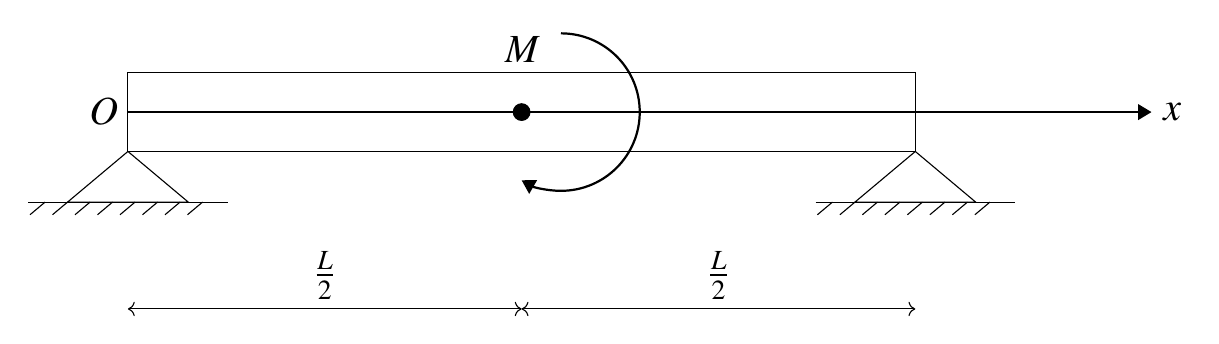
\begin{tikzpicture}
		\draw (0, 0) rectangle (10, 1);
		\draw[-Triangle, thick] (0, 0.5) -- (13, 0.5);
		\node at (0, 0.5) [left] {\Large $O$};
		\filldraw (5,0.5) circle[radius=3pt];
		\node at (5, 1) [above] {\Large $M$};
		\node at (13, 0.5) [right] {\Large $x$};
		\draw ({-cos(40)}, {-sin(40)}) -- (0, 0) -- ({cos(40)}, {-sin(40)}) -- cycle;
		\draw ({10-cos(40)}, {-sin(40)}) -- (10, 0) -- ({10+cos(40)}, {-sin(40)}) -- cycle;
		\draw [-Triangle, thick] (5.5, 1.5) arc (90:-120:1);

		\draw ({-0.5-cos(40)}, {-sin(40)}) -- ({0.5+cos(40)}, {-sin(40)});
		\foreach \x in {-1,...,6}
		\draw ({\x/3.5 - cos(40)}, {- sin(40)}) -- ({\x/3.5 - 1.25*cos(40)}, {-1.25*sin(40)});

		\draw ({10-0.5-cos(40)}, {-sin(40)}) -- ({10 + 0.5+cos(40)}, {-sin(40)});
		\foreach \x in {-1,...,6}
		\draw ({10 + \x/3.5 - cos(40)}, {- sin(40)}) -- ({10 + \x/3.5 - 1.25*cos(40)}, {-1.25*sin(40)});

		\draw [<->] (0, -2) -- (5, -2);
		\node at (2.5, -2) [above] {\Large $\frac{L}{2}$};

		\draw [<->] (5, -2) -- (10, -2);
		\node at (7.5, -2) [above] {\Large $\frac{L}{2}$};
	\end{tikzpicture}
	\end{center}
	\begin{enumerate}
		\item 
		\begin{center}
		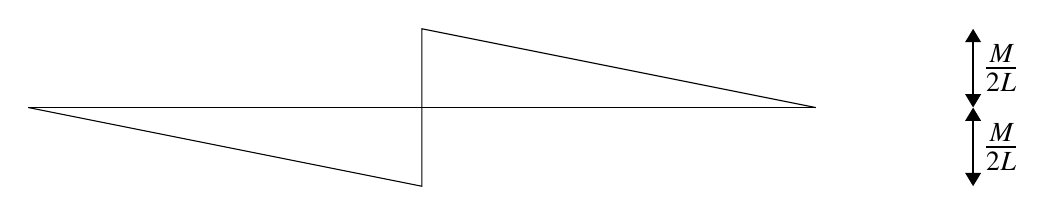
\begin{tikzpicture}
			\draw (0, 0) -- (10, 0);
			\draw (0, 0) -- (5, -1) -- (5, 1) -- (10, 0);

			\draw [Triangle-Triangle, thick] (12, 0) -- (12, 1);
			\node at (12, 0.5) [right] {\Large $\frac{M}{2L}$};

			\draw [Triangle-Triangle, thick] (12, 0) -- (12, -1);
			\node at (12, -0.5) [right] {\Large $\frac{M}{2L}$};
		\end{tikzpicture}
		\end{center}
		\item
		\begin{center}
		\begin{tikzpicture}
			\draw (0, 0) -- (10, 0);
			\draw (0, 0) -- (0, -1) -- (5, -1) -- (5, 1) -- (10, 1) -- (10, 0);

			\draw [Triangle-Triangle, thick] (12, 0) -- (12, 1);
			\node at (12, 0.5) [right] {\Large $\frac{M}{2L}$};

			\draw [Triangle-Triangle, thick] (12, 0) -- (12, -1);
			\node at (12, -0.5) [right] {\Large $\frac{M}{2L}$};
		\end{tikzpicture}
		\end{center}
		\item
		\begin{center}
		\begin{tikzpicture}
			\draw (0, 0) -- (0, 2) -- (10, 2) -- (10, 0) -- cycle;

			\draw [Triangle-Triangle, thick] (12, 0) -- (12, 2);
			\node at (12, 1) [right] {\Large $\frac{M}{L}$};
		\end{tikzpicture}
		\end{center}
		\item
		\begin{center}
		\begin{tikzpicture}
			\draw (0, 0) -- (0, 1) -- (10, 1) -- (10, 0) -- cycle;

			\draw [Triangle-Triangle, thick] (12, 0) -- (12, 1);
			\node at (12, 0.5) [right] {\Large $\frac{M}{2L}$};
		\end{tikzpicture}
		\end{center}
	\end{enumerate}

	%Question67
	\item An idealized thin-walled cross-section of a beam and the respective areas of the booms are shown. A bending moment $M_y$ is acting on the cross-section. The ratio of the magnitude of normal stress in the top booms to that of the bottom boom is
	\begin{center}
	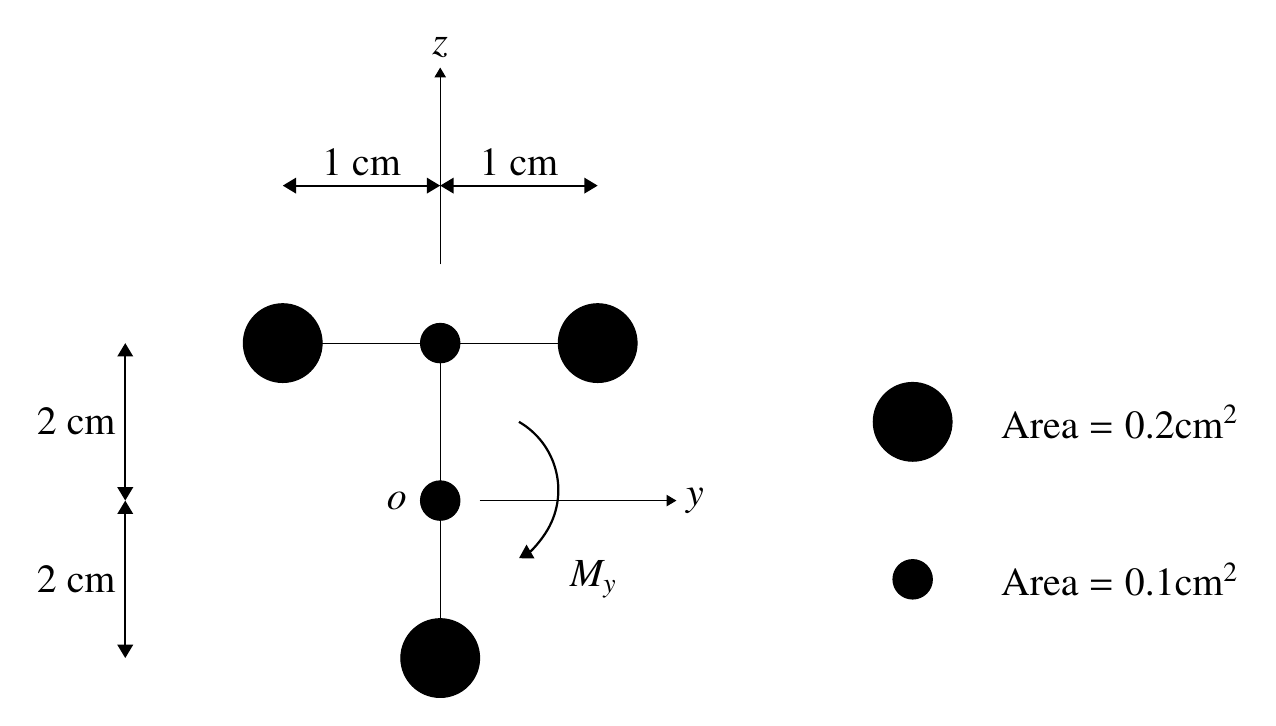
\begin{tikzpicture}
		\filldraw (0,0) circle[radius=0.25cm];
		\draw (0, -2) -- (0, 2);
		\filldraw (0,-2) circle[radius=0.5cm];
		\filldraw (0,2) circle[radius=0.25cm];
		\draw (-2, 2) -- (2, 2);
		\filldraw (2,2) circle[radius=0.5cm];
		\filldraw (-2,2) circle[radius=0.5cm];

		\draw [-Triangle] (0.5, 0) -- (3, 0);
		\node at (3, 0) [right] {\Large $y$};

		\draw [-Triangle] (0, 3) -- (0, 5.5);
		\node at (0, 5.5) [above] {\Large $z$};

		\draw [Triangle-Triangle, thick] (-4, 0) -- (-4, 2);
		\node at (-4, 1) [left] {\Large $2$ cm};

		\draw [Triangle-Triangle, thick] (-4, 0) -- (-4, -2);
		\node at (-4, -1) [left] {\Large $2$ cm};

		\draw [Triangle-Triangle, thick] (-2, 4) -- (0, 4);
		\node at (-1, 4) [above] {\Large $1$ cm};

		\draw [Triangle-Triangle, thick] (0, 4) -- (2, 4);
		\node at (1, 4) [above] {\Large $1$ cm};

		\node at (0, 0) [left=3mm] {\Large $o$};
		\node at (1.5, -1) [right] {\Large $M_y$};

		\draw [-Triangle, thick] (1, 1) arc (60:-60:1);

		\node at (7, 1) [right] {\Large Area $= 0.2 \text{cm}^2$};
		\filldraw (6,1) circle[radius=0.5cm];

		\node at (7, -1) [right] {\Large Area $= 0.1 \text{cm}^2$};
		\filldraw (6, -1) circle[radius=0.25cm];
		
	\end{tikzpicture}
	\end{center}
	\begin{enumerate}
		\item $\frac{5}{11}$
		\item $\frac{2}{5}$
		\item $1$
		\item $\frac{5}{2}$
	\end{enumerate}

	%Question68
	\item An engineer is asked to test a system which can be idealized as SDOF \brak{\text{single degree of freedom}} with viscous damping. A frequency response test was conducted and it is found that the quality factor $Q$ is equal to $10$. What will be the logarithmic decrement if a free vibration test is performed?
	\begin{enumerate}
		\item $\frac{\pi}{40}$
		\item $\frac{\pi}{20}$
		\item $\frac{\pi}{10}$
		\item $\frac{\pi}{5}$
	\end{enumerate}

\end{enumerate}
\end{document}
